\documentclass[11pt,a4paper]{article}
\usepackage{iftex}
\ifPDFTeX
  \usepackage[utf8]{inputenc}
  \usepackage[T1]{fontenc}
\else
  \usepackage{fontspec}
  \setmainfont{lmroman10-regular.otf}[
    BoldFont=lmroman10-bold.otf,
    ItalicFont=lmroman10-italic.otf,
    BoldItalicFont=lmroman10-bolditalic.otf]
\fi
\usepackage[margin=2.5cm]{geometry}
\usepackage{amsmath,amssymb}
\usepackage{booktabs}
\usepackage{graphicx}
\usepackage{microtype}
\usepackage[hidelinks]{hyperref}

\title{Mathematical Formulation of the Main Line}
\author{}
\date{}

\begin{document}
\maketitle

\section{Introduction}
\label{sec:A}
MobiPhlex is responsible for developing the mobile telecommunications network in southwestern Poland. The assignment considers two phases of this development: constructing a main line from Warszawa to Jelenia Góra, and subsequently connecting the cities outside the main line to switching stations in Warszawa, Kielce, and Opole. The formulation presented here addresses the first phase, in which the cities visited and the connections constructed must be chosen to minimize construction cost while satisfying geographic and government requirements.

The main line passes through three areas in sequence. In area 1, it runs from Warszawa to Radom; in area 2, from Kielce to Gliwice; and in area 3, from Opole to Jelenia Góra. The existing Radom--Kielce and Gliwice--Opole connections must be used to join these paths. Besides the endpoints, the line must visit at least two cities in area 1 and at least three cities in each of areas 2 and 3.

The government imposes additional requirements on city selection. At least one of Konin and Kalisz must be included, and at least one of Poznań, Zielona Góra, and Leszno must be included. At most one of Bytom, Sosnowiec, and Katowice may be visited, and Wodzisław Śląski and Jastrzębie-Zdrój cannot both be visited. These requirements apply to the complete main line, irrespective of area. A connection between two cities may not be selected in both directions.

\subsection{Modeling assumptions}
The following assumptions specify how the case is represented mathematically:
\begin{enumerate}
  \item \textbf{Distances and construction costs.} New cable follows a straight line between connected cities, so its length is the Euclidean distance between their coordinates. Roads, terrain, and obstacles are ignored. Construction cost per coordinate unit is assumed to be identical for all new connections. The unit cost is normalized to one, making minimum cost equivalent to minimum new cable length.
  \item \textbf{Available connections.} Any pair of distinct cities within the same area may be connected. The only connections permitted between areas are the two existing links specified in the case. These links are assumed to be available without additional construction cost.
  \item \textbf{Route structure.} The main line is interpreted as a single continuous path, without branches, disconnected cycles, or repeated cities. Each area is visited as one block, in the order area 1, area 2, then area 3. The specified starting and ending cities of each area are mandatory.
  \item \textbf{Intermediate-city counts.} The requirement to visit two or three additional cities is interpreted as a minimum rather than an exact count. The starting and ending cities do not count toward these minimums.
  \item \textbf{Direction of connections.} Directed connections represent the visiting order along the main line. They do not imply one-way transmission: information can travel in both directions through the physical cable.
  \item \textbf{Data and capacity.} City coordinates and area assignments are treated as fixed and accurate. No main cable capacity restriction is imposed, because the case specifies no such limit. City demand and switching-station capacities are reserved for the second-phase connection model.
\end{enumerate}

The main line problem is represented by a binary integer linear program that selects cities and connections. The intended route is continuous, but the formulation can permit disconnected cycles involving three or more cities. The computed solution must therefore be checked to establish that all selected cities belong to the main line.

\subsection{Comparison of assumptions with AI suggestions}
\textit{To be completed by the authors: describe the assumptions written before using AI, identify which assumptions were changed after reviewing AI suggestions, and explain which suggestions were rejected and why. Use the actual project history and record these decisions in the AI log.}

\section{Mathematical formulation -- Main line}
\subsection{Sets and parameters}

Let $K=\{1,2,3\}$ denote the geographic areas. For each $k\in K$, define:
\begin{description}
  \item[$V_k$] The set of cities in area $k$.
  \item[$s_k,t_k$] The starting and ending cities of area $k$.
  \item[$I_k$] The intermediate cities, $I_k=V_k\setminus\{s_k,t_k\}$.
  \item[$A_k$] The possible directed connections, $A_k=\{(i,j)\in V_k\times V_k:i\ne j\}$.
  \item[$R_k$] The minimum number of intermediate cities, with $R_1=2$ and $R_2=R_3=3$.
\end{description}

\begin{center}
\begin{tabular}{lll}
\toprule
Area $k$ & Start $s_k$ & End $t_k$\\
\midrule
1 & Warszawa & Radom\\
2 & Kielce & Gliwice\\
3 & Opole & Jelenia Góra\\
\bottomrule
\end{tabular}
\end{center}

Let $V=\bigcup_{k\in K}V_k$. For every city $i\in V$, $(X_i,Y_i)$ are its coordinates. The distance between cities is the fixed parameter
\begin{equation}
d_{ij}=\sqrt{(X_i-X_j)^2+(Y_i-Y_j)^2}.
\end{equation}
Let $c$ denote the uniform construction cost per coordinate unit. In the implementation, $c=1$, so the objective measures new cable length.

\subsection{Decision variables}
For every $(i,j)\in A_k$, $k\in K$, define
\[
x_{ij}=\begin{cases}
1,&\text{if connection $i\rightarrow j$ is selected},\\
0,&\text{otherwise}.
\end{cases}
\]
For every $i\in V$, define
\[
y_i=\begin{cases}
1,&\text{if city $i$ is included in the main line},\\
0,&\text{otherwise}.
\end{cases}
\]
A connection's direction represents visiting order; the physical cable permits information to travel in both directions.

\subsection{Objective function}
Minimize the construction cost of new cable:
\begin{equation}
\min\quad c\sum_{k\in K}\sum_{(i,j)\in A_k}d_{ij}x_{ij}.
\label{eq:objective}
\end{equation}
The existing connections are excluded because they require no new construction.

\subsection{Constraints}
\subsubsection{Route requirements}
The starting city has exactly one outgoing connection and no incoming connection:
\begin{align}
\sum_{j\in V_k\setminus\{s_k\}}x_{s_kj}&=1 &&\forall k\in K,\\
\sum_{i\in V_k\setminus\{s_k\}}x_{is_k}&=0 &&\forall k\in K.
\end{align}
The ending city has exactly one incoming connection and no outgoing connection:
\begin{align}
\sum_{i\in V_k\setminus\{t_k\}}x_{it_k}&=1 &&\forall k\in K,\\
\sum_{j\in V_k\setminus\{t_k\}}x_{t_kj}&=0 &&\forall k\in K.
\end{align}
Both endpoints must be included:
\begin{equation}
y_{s_k}=y_{t_k}=1\qquad\forall k\in K.
\end{equation}
Each selected intermediate city has exactly one outgoing and one incoming connection. An unselected city has neither:
\begin{align}
\sum_{j\in V_k\setminus\{i\}}x_{ij}&=y_i &&\forall k\in K,\ i\in I_k,\\
\sum_{j\in V_k\setminus\{i\}}x_{ji}&=y_i &&\forall k\in K,\ i\in I_k.
\end{align}
The minimum number of intermediate cities is enforced by
\begin{equation}
\sum_{i\in I_k}y_i\ge R_k\qquad\forall k\in K.
\end{equation}

\subsubsection{Government requirements}
At least one of Konin and Kalisz must be included:
\begin{equation}
y_{\text{Konin}}+y_{\text{Kalisz}}\ge1.
\end{equation}
At most one of Bytom, Sosnowiec, and Katowice may be included:
\begin{equation}
y_{\text{Bytom}}+y_{\text{Sosnowiec}}+y_{\text{Katowice}}\le1.
\end{equation}
Wodzisław Śląski and Jastrzębie-Zdrój cannot both be included:
\begin{equation}
y_{\text{Wodzisław Śląski}}+y_{\text{Jastrzębie-Zdrój}}\le1.
\end{equation}
At least one of Poznań, Zielona Góra, and Leszno must be included:
\begin{equation}
y_{\text{Poznań}}+y_{\text{Zielona Góra}}+y_{\text{Leszno}}\ge1.
\end{equation}

\subsubsection{Connection restriction}
To prohibit selecting both directions between the same pair of cities, impose
\begin{equation}
x_{ij}+x_{ji}\le1
\qquad\forall k\in K,\ i,j\in V_k,\ i<j.
\end{equation}
Here, $i<j$ refers to an arbitrary fixed ordering of cities, so each unordered pair is considered once.

\subsubsection{Variable domains}
\begin{align}
x_{ij}&\in\{0,1\} &&\forall k\in K,\ (i,j)\in A_k,\\
y_i&\in\{0,1\} &&\forall i\in V.
\end{align}
The fixed existing connections join the endpoint paths into a main line from Warszawa to Jelenia Góra. The connection restriction prevents two-city cycles, but disconnected cycles involving three or more cities remain possible. Verification must therefore check both the path from the start to the end and whether any selected connections lie outside that path.

\section{Implementation -- Main line}
\subsection{Implementation and data}
The model was implemented in Python using Gurobi 13.0.3. The script \texttt{c\_model.py} reads city names, area assignments, and coordinates from \texttt{cities.csv}, calculates Euclidean distances, and creates the binary connection and city-selection variables. Area endpoints, minimum city counts, and government selection rules are specified in the script. City demands are not used in this phase. The current implementation reads city data from a file but hard-codes the other case parameters; moving those parameters into an input file remains necessary to satisfy the assignment's requirement that all data be read from files.

The objective minimizes the total length of new cable. After optimization, the script follows the selected outgoing connections from each area's starting city to its ending city. It prints the objective value and the ordered route, and saves the route to \texttt{c\_solution.csv}. The existing Radom--Kielce and Gliwice--Opole links join the three area paths and are excluded from new cable length.

The solver log records 196 constraints and 256 variables, of which 230 are binary. The remaining 26 continuous variables are auxiliary variables retained in the implementation; their bounds do not restrict the cable-selection decisions. Gurobi removes them during presolve. The mathematical formulation therefore presents only the variables relevant to route selection.

\subsection{Results of the normal run}
Gurobi reported an optimal solution with objective value $130.998$ coordinate units, displayed by the script as $131.00$. The reported optimality gap was $0.00\%$, and the solve time was approximately $0.03$ seconds on the machine used. The route includes 14 cities, with the area paths shown in Table~\ref{tab:normal-route}.

\begin{table}[htbp]
\centering
\small
\begin{tabular}{p{0.07\textwidth}p{0.65\textwidth}r}
\toprule
Area & Cities in visiting order & Length\\
\midrule
1 & Warszawa $\rightarrow$ Skierniewice $\rightarrow$ Piotrków $\rightarrow$ Radom & 32.98\\
2 & Kielce $\rightarrow$ Kraków $\rightarrow$ Bielsko $\rightarrow$ Jastrzębie-Zdrój $\rightarrow$ Gliwice & 43.32\\
3 & Opole $\rightarrow$ Kalisz $\rightarrow$ Leszno $\rightarrow$ Legnica $\rightarrow$ Jelenia Góra & 54.70\\
\midrule
 & Total new cable & 131.00\\
\bottomrule
\end{tabular}
\caption{Main line route and new cable lengths from the normal run. Lengths are expressed in coordinate units and rounded to two decimal places.}
\label{tab:normal-route}
\end{table}

Concatenating the paths in Table~\ref{tab:normal-route}, with the two existing links between them, gives the complete route from Warszawa to Jelenia Góra. Area 1 includes two intermediate cities, while areas 2 and 3 each include three. Kalisz satisfies the Konin/Kalisz requirement, and Leszno satisfies the Poznań/Zielona Góra/Leszno requirement. None of Bytom, Sosnowiec, and Katowice is visited. Jastrzębie-Zdrój is visited while Wodzisław Śląski is excluded.

\subsection{Visualization and independent verification}
The script \texttt{c\_visualize.py} draws the saved route using the supplied coordinates. New connections are colored by area, existing links are dashed, and selected cities are numbered in visiting order. The resulting map is saved as \texttt{c\_map.png} and shown in Figure~\ref{fig:normal-map}. The visualization shows a continuous route with no repeated cities or disconnected components.

\begin{figure}[htbp]
\centering
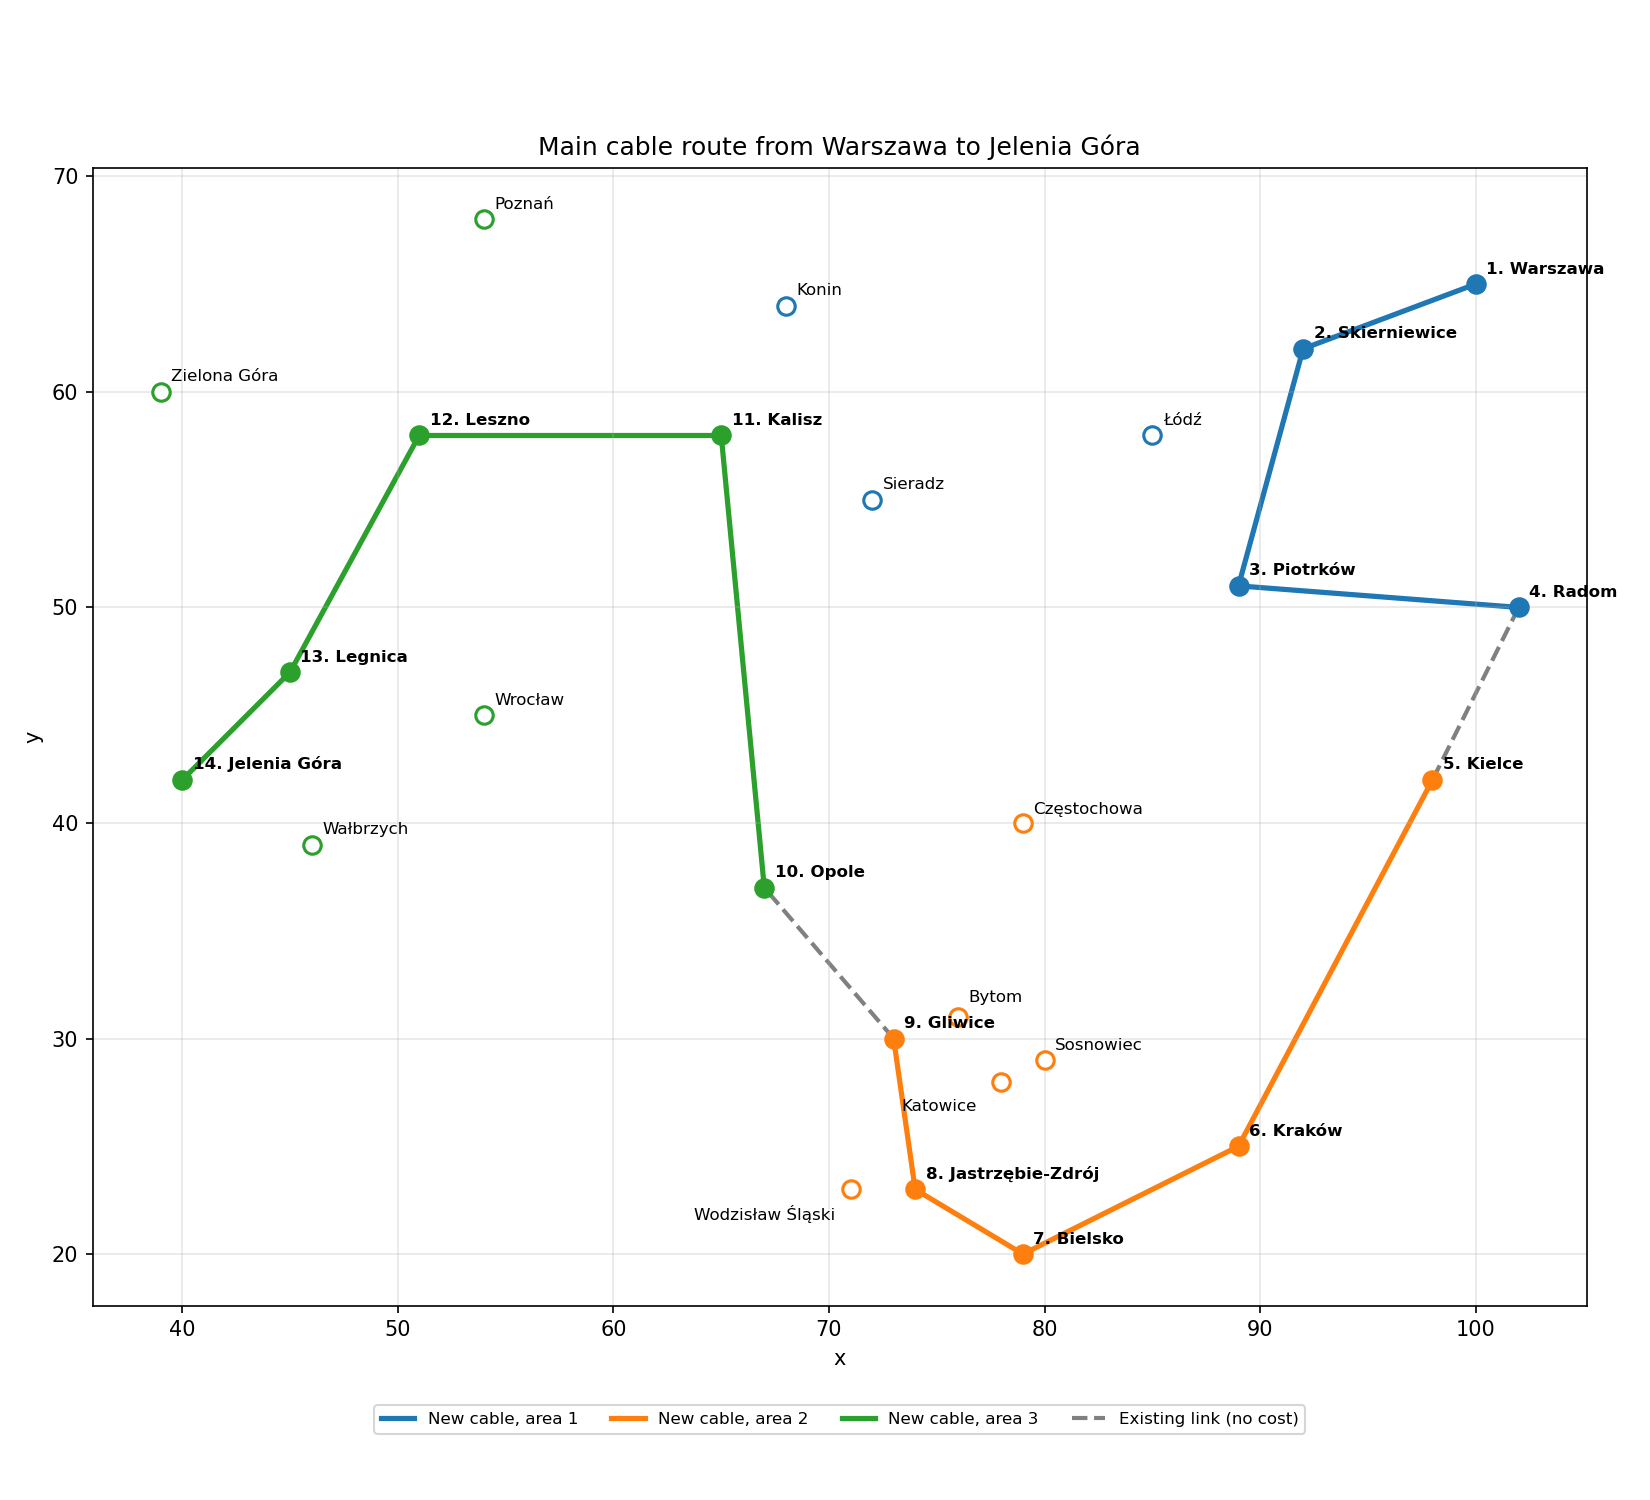
\includegraphics[width=\textwidth,height=0.75\textheight,keepaspectratio]{src/results/c_map.png}
\caption{Main line from the normal run. Numbers indicate visiting order, filled markers identify selected cities, and dashed gray lines represent the existing links. The total new cable length is $130.998$ coordinate units.}
\label{fig:normal-map}
\end{figure}

The checker \texttt{c\_check.py} reads the city data and saved route without importing the optimization model. It checks the endpoints, area order, intermediate-city counts, existing links, government requirements, repeated cities, and agreement with the input coordinates. The saved route passed all 27 checks, and its independently calculated new cable length was $130.998$ coordinate units.

\textit{To be completed by the authors: document how the checker was generated, including the prompt and whether the AI received only the case text and solution-file format, without access to the model. Not importing the model does not by itself establish the independent generation required by the assignment.}

These checks establish feasibility of the exported route. Because the normal output file contains only the extracted path, the checker alone cannot rule out additional selected connections omitted from that file. However, the summed new cable length of the exported path agrees with the solver's objective value. All candidate new connections in this dataset have strictly positive lengths, so this agreement also rules out additional selected connections for the reported solution, within numerical precision. Gurobi's optimality result applies to the implemented formulation; combined with the verified continuous route, it establishes an optimal valid main line for this dataset.

\subsection{Experiment without the two-way restriction}
To investigate the role of the two-way restriction, the model was solved again using \texttt{c\_model\_broken.py} with \texttt{USE\_ONE\_DIRECTION = False}. The restriction $x_{ij}+x_{ji}\le1$ was omitted, while the other constraints of the normal run were retained. This reduced the number of constraints from 196 to 94.

Gurobi reported an optimal objective value of $122.458$ coordinate units, with a $0.00\%$ gap and an approximate solve time of $0.02$ seconds. This objective includes every selected directed connection, including connections in disconnected cycles. It does not represent the length of a valid continuous main line.

\begin{table}[htbp]
\centering
\small
\begin{tabular}{p{0.07\textwidth}p{0.65\textwidth}r}
\toprule
Area & Extracted endpoint path & Length\\
\midrule
1 & Warszawa $\rightarrow$ Radom & 15.13\\
2 & Kielce $\rightarrow$ Bytom $\rightarrow$ Gliwice & 27.76\\
3 & Opole $\rightarrow$ Wrocław $\rightarrow$ Leszno $\rightarrow$ Legnica $\rightarrow$ Jelenia Góra & 48.21\\
\midrule
 & Total endpoint-path length & 91.10\\
\bottomrule
\end{tabular}
\caption{Endpoint paths in the broken run. Lengths exclude disconnected cycles and existing links and are rounded to two decimal places.}
\label{tab:broken-route}
\end{table}

In addition to the paths in Table~\ref{tab:broken-route}, the model selected
\[
\text{Konin}\rightarrow\text{Sieradz}\rightarrow\text{Konin}
\]
and
\[
\text{Bielsko}\rightarrow\text{Jastrzębie-Zdrój}\rightarrow\text{Bielsko}.
\]
Each Konin--Sieradz arc has length approximately $9.85$, and each Bielsko--Jastrzębie-Zdrój arc has length approximately $5.83$. Both directions contribute separately to the broken model's objective. The script saves all selected connections in \texttt{c\_broken\_arcs.csv}; \texttt{c\_visualize\_broken.py} draws them in \texttt{c\_broken\_map.png}, highlighting the two-way connections in red.

The disconnected cycles allow the model to satisfy city-selection constraints without visiting those cities on the main path. In area 1, Konin and Sieradz satisfy the count of two intermediate cities, although the endpoint path visits none. Konin also satisfies the Konin/Kalisz selection constraint despite being disconnected. In area 2, Bytom, Bielsko, and Jastrzębie-Zdrój satisfy the count of three intermediate cities, although only Bytom lies on the endpoint path. Thus, the lower objective is achieved by violating the intended meaning of a continuous main line.

Figure~\ref{fig:broken-map} shows the broken solution. The red segments each represent two selected directed connections drawn on top of one another.

\begin{figure}[htbp]
\centering
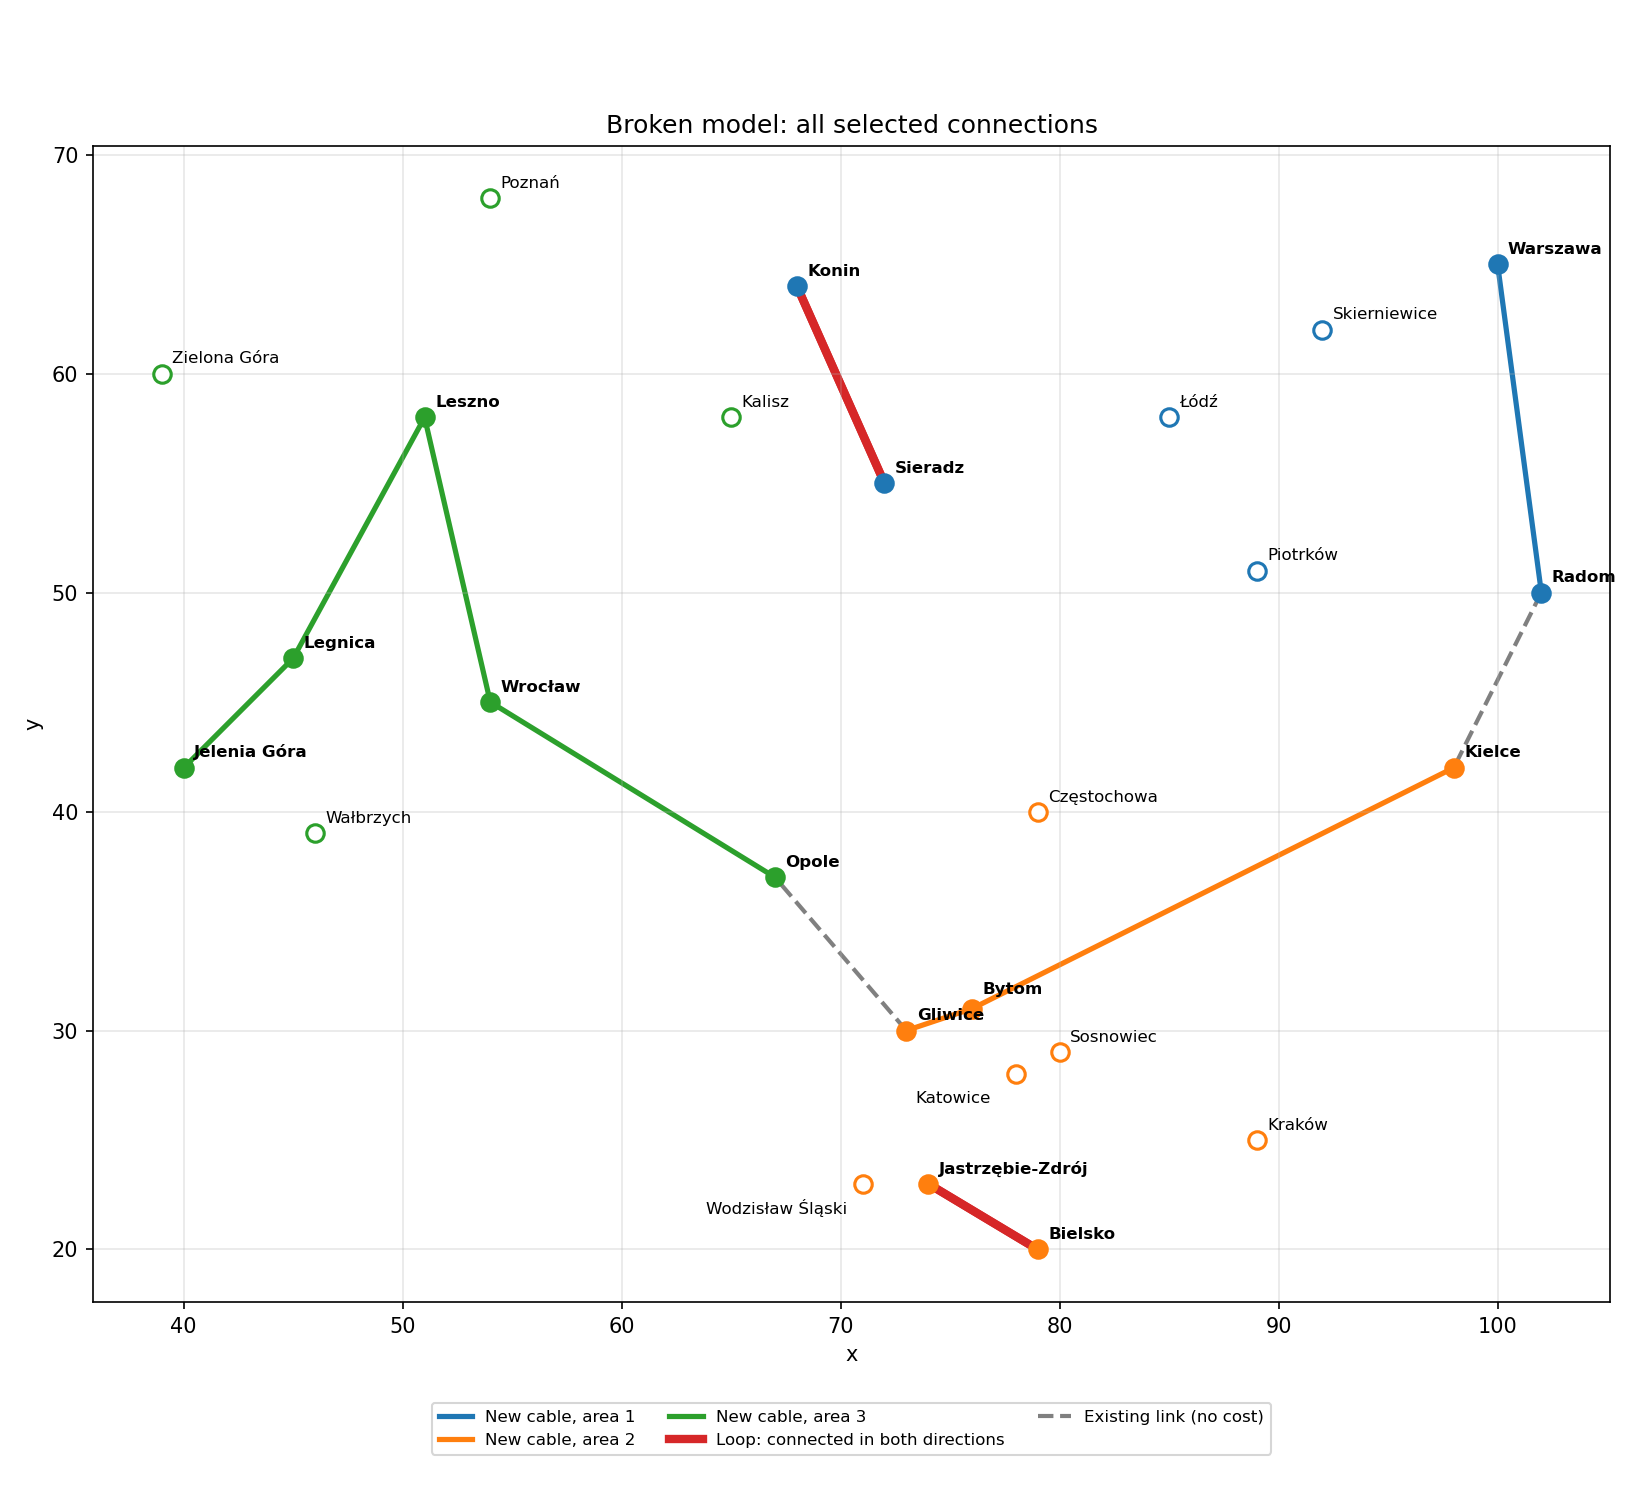
\includegraphics[width=\textwidth,height=0.75\textheight,keepaspectratio]{src/results/c_broken_map.png}
\caption{Selected connections when the two-way restriction is removed. The disconnected Konin--Sieradz and Bielsko--Jastrzębie-Zdrój cycles are highlighted in red. The objective is $122.458$ coordinate units, including both directions of each cycle, but the solution is not a valid continuous main line.}
\label{fig:broken-map}
\end{figure}

\subsection{Interpretation and limitations}
The broken objective is approximately $8.54$ coordinate units lower than the normal objective. The experiment shows that the two-way restriction prevents disconnected two-city cycles that would otherwise count toward the required city visits.

However, this restriction is not sufficient for all possible city coordinates. A disconnected cycle involving three or more cities can satisfy the incoming and outgoing degree constraints without selecting both directions of any connection. For example, three optional cities located close together but far from the endpoint path could form a cheap disconnected triangle. The normal run produces a valid continuous solution for the supplied data, but the formulation does not guarantee connectivity for arbitrary instances. It is therefore a relaxation of the intended continuous-path problem, rather than a complete formulation of that requirement. Verification confirms the reported solution, but does not repair this general modeling limitation.

\section{Mathematical formulation -- Connecting cities}
\label{sec:copper-model}
The second phase connects cities outside the main line to switching stations in Warszawa, Kielce, and Opole. The main line obtained in the first phase is treated as fixed. Cable capacity may be purchased in any nonnegative quantity, and construction cost is proportional to both distance and capacity. The resulting model is a continuous linear program.

\subsection{Sets and parameters}
Let $V^{\mathrm{main}}$ be the cities visited by the selected main line, and define
\[
N=V\setminus V^{\mathrm{main}},
\qquad S=\{\text{Warszawa},\text{Kielce},\text{Opole}\}.
\]
Thus, $N$ contains the cities requiring copper connections, and $S$ contains the switching stations. Connections to stations in other geographic areas are permitted.

For each $i\in N$, let $q_i$ be its demand in TB/s. The cable length from city $i$ to station $s$ is
\begin{equation}
d_{is}=\sqrt{(X_i-X_s)^2+(Y_i-Y_s)^2}.
\end{equation}
Let $B_s$ denote the available station capacity, with
\[
B_{\text{Warszawa}}=800,\qquad
B_{\text{Kielce}}=1200,\qquad
B_{\text{Opole}}=400
\quad\text{TB/s}.
\]
These capacities correspond to two, three, and one standard units, respectively, each with capacity 400 TB/s. Let $c^{\mathrm{Cu}}=1000$ denote the cable price in EUR per coordinate unit and TB/s.

To exclude connections with no positive distance-dependent capacity, define the eligible pairs
\[
E=\{(i,s)\in N\times S:d_{is}<70\}.
\]
For each $(i,s)\in E$, define the fixed capacity bound
\begin{equation}
U_{is}=\min\{200,\;2\pi\min(35,70-d_{is})\}.
\label{eq:copper-bound}
\end{equation}
This combines the maximum cable capacity of 200 TB/s with the distance-dependent limit. Distances and bounds are calculated before optimization. Write $S_i=\{s\in S:(i,s)\in E\}$ and $N_s=\{i\in N:(i,s)\in E\}$.

\subsection{Decision variables}
For every $(i,s)\in E$, let
\[
f_{is}\in\mathbb{R}_{\ge0}
\]
be the installed cable capacity between city $i$ and station $s$, measured in TB/s. Capacity is allocated to carry the city's demand; no unnecessary spare capacity is purchased. A zero value means that no cable is installed. Each city--station pair represents a single cable, so parallel cables cannot be used to circumvent its capacity bound.

\subsection{Objective function}
Minimize the total cost of copper connections:
\begin{equation}
\min\quad c^{\mathrm{Cu}}\sum_{(i,s)\in E}d_{is}f_{is}.
\label{eq:copper-objective}
\end{equation}
The objective is measured in EUR. For example, a cable of length 3.4 coordinate units and capacity 80 TB/s costs $1000\times3.4\times80=272{,}000$ EUR.

\subsection{Constraints}
Each city must receive sufficient cable capacity to carry its demand:
\begin{equation}
\sum_{s\in S_i}f_{is}=q_i
\qquad\forall i\in N.
\label{eq:copper-demand}
\end{equation}
Equality reflects the assumption that no spare capacity is purchased. With positive connection costs, using a lower bound instead would also give exact demand satisfaction at an optimum.

The total capacity allocated to a station cannot exceed its installed capacity:
\begin{equation}
\sum_{i\in N_s}f_{is}\le B_s
\qquad\forall s\in S.
\label{eq:copper-station}
\end{equation}

Every cable must satisfy both its physical capacity limit and its distance-dependent limit:
\begin{equation}
f_{is}\le U_{is}
\qquad\forall(i,s)\in E.
\label{eq:copper-capacity}
\end{equation}

If Łódź belongs to $N$, no single cable may carry more than 40\% of its total outgoing flow. By constraint~\eqref{eq:copper-demand}, that flow equals its demand, giving
\begin{equation}
f_{\text{Łódź},s}\le0.4q_{\text{Łódź}}
\qquad\forall s\in S_{\text{Łódź}}.
\label{eq:copper-lodz}
\end{equation}
For the supplied demand of 317 TB/s, this bound is 126.8 TB/s per cable. With only three switching stations, meeting this demand requires a positive connection to all three.

Finally, capacities are continuous and nonnegative:
\begin{equation}
f_{is}\ge0\qquad\forall(i,s)\in E.
\end{equation}
No binary installation variables are required because there is no fixed connection charge or minimum cable capacity. Although equation~\eqref{eq:copper-bound} contains minimum expressions, these define fixed parameters; the objective and all constraints are linear in the decision variables.

\section{Implementation and results -- Connecting cities}
\label{sec:copper-results}
\subsection{Implementation}
The continuous linear program was implemented in \texttt{e\_model.py} using Python and Gurobi 13.0.3. City coordinates and demands are read from \texttt{cities.csv}, while station capacities and cable parameters are read from \texttt{copper\_parameters.json}. The fixed main line is read from \texttt{c\_solution.csv}. Only cities outside that route require copper connections.

For the main line obtained in the first phase, 12 cities require connections. All 36 city--station pairs have positive distance-dependent capacity. The implemented LP has 36 continuous variables and 54 constraints. Gurobi reported an optimal solution after 10 simplex iterations. Capacities and connection costs are saved in \texttt{e\_solution.csv}, station utilization in \texttt{e\_stations.csv}, and dual values in \texttt{e\_duals.csv}.

\subsection{Minimum connection cost and cable capacities}
The minimum cost of connecting the remaining cities is
\[
\boxed{66{,}696{,}434.43\ \text{EUR}.}
\]
This cost covers only the second-phase copper connections. It excludes the construction cost of the main line. The solution purchases 22 positive-capacity cables and meets a total demand of 2331 TB/s.

\begin{table}[htbp]
\centering
\small
\begin{tabular}{lrrr}
\toprule
City & Warszawa & Kielce & Opole\\
\midrule
Łódź & 126.800 & 126.800 & 63.400\\
Konin & 200.000 & 36.000 & 0.000\\
Sieradz & 118.864 & 59.136 & 0.000\\
Częstochowa & 78.000 & 200.000 & 0.000\\
Bytom & 0.000 & 163.000 & 0.000\\
Sosnowiec & 0.000 & 143.000 & 0.000\\
Katowice & 1.890 & 200.000 & 61.110\\
Wodzisław Śląski & 0.000 & 119.000 & 0.000\\
Poznań & 150.182 & 100.818 & 0.000\\
Zielona Góra & 55.263 & 52.247 & 13.490\\
Wrocław & 0.000 & 0.000 & 133.000\\
Wałbrzych & 0.000 & 0.000 & 129.000\\
\midrule
Total & 731.000 & 1200.000 & 400.000\\
\bottomrule
\end{tabular}
\caption{Installed copper cable capacities in TB/s. Values are rounded to three decimal places; zero indicates that no cable is installed.}
\label{tab:copper-capacities}
\end{table}

In particular, Poznań requires 150.182 TB/s to Warszawa and 100.818 TB/s to Kielce, with no connection to Opole. Wałbrzych requires 129.000 TB/s to Opole and no capacity to the other stations. The Warszawa connection from Poznań reaches its distance-dependent upper bound. Łódź is connected to all three stations: its cables to Warszawa and Kielce each carry 40\% of its demand, while its cable to Opole carries the remaining 20\%.

\subsection{Switching-station utilization}
\begin{table}[htbp]
\centering
\begin{tabular}{lrrr}
\toprule
Station & Available (TB/s) & Used (TB/s) & Utilization\\
\midrule
Warszawa & 800 & 731 & 91.375\%\\
Kielce & 1200 & 1200 & 100.000\%\\
Opole & 400 & 400 & 100.000\%\\
\bottomrule
\end{tabular}
\caption{Capacity utilization at the switching stations.}
\label{tab:copper-stations}
\end{table}
The station in Kielce is fully utilized: 1200 of its available 1200 TB/s are allocated. Opole is also fully utilized, while Warszawa has 69 TB/s of unused capacity. Overall, 2331 of the available 2400 TB/s are utilized. Unused capacity at Warszawa does not imply that every city could increase its allocation there, because individual cables also have capacity and distance restrictions.

\subsection{Visualization and verification}
The script \texttt{e\_visualize.py} produces a separate panel for each switching station. Copper cables are labeled with their installed capacities, while the fixed main line is shown in gray. Figure~\ref{fig:copper-map} displays the resulting allocation.

\begin{figure}[htbp]
\centering
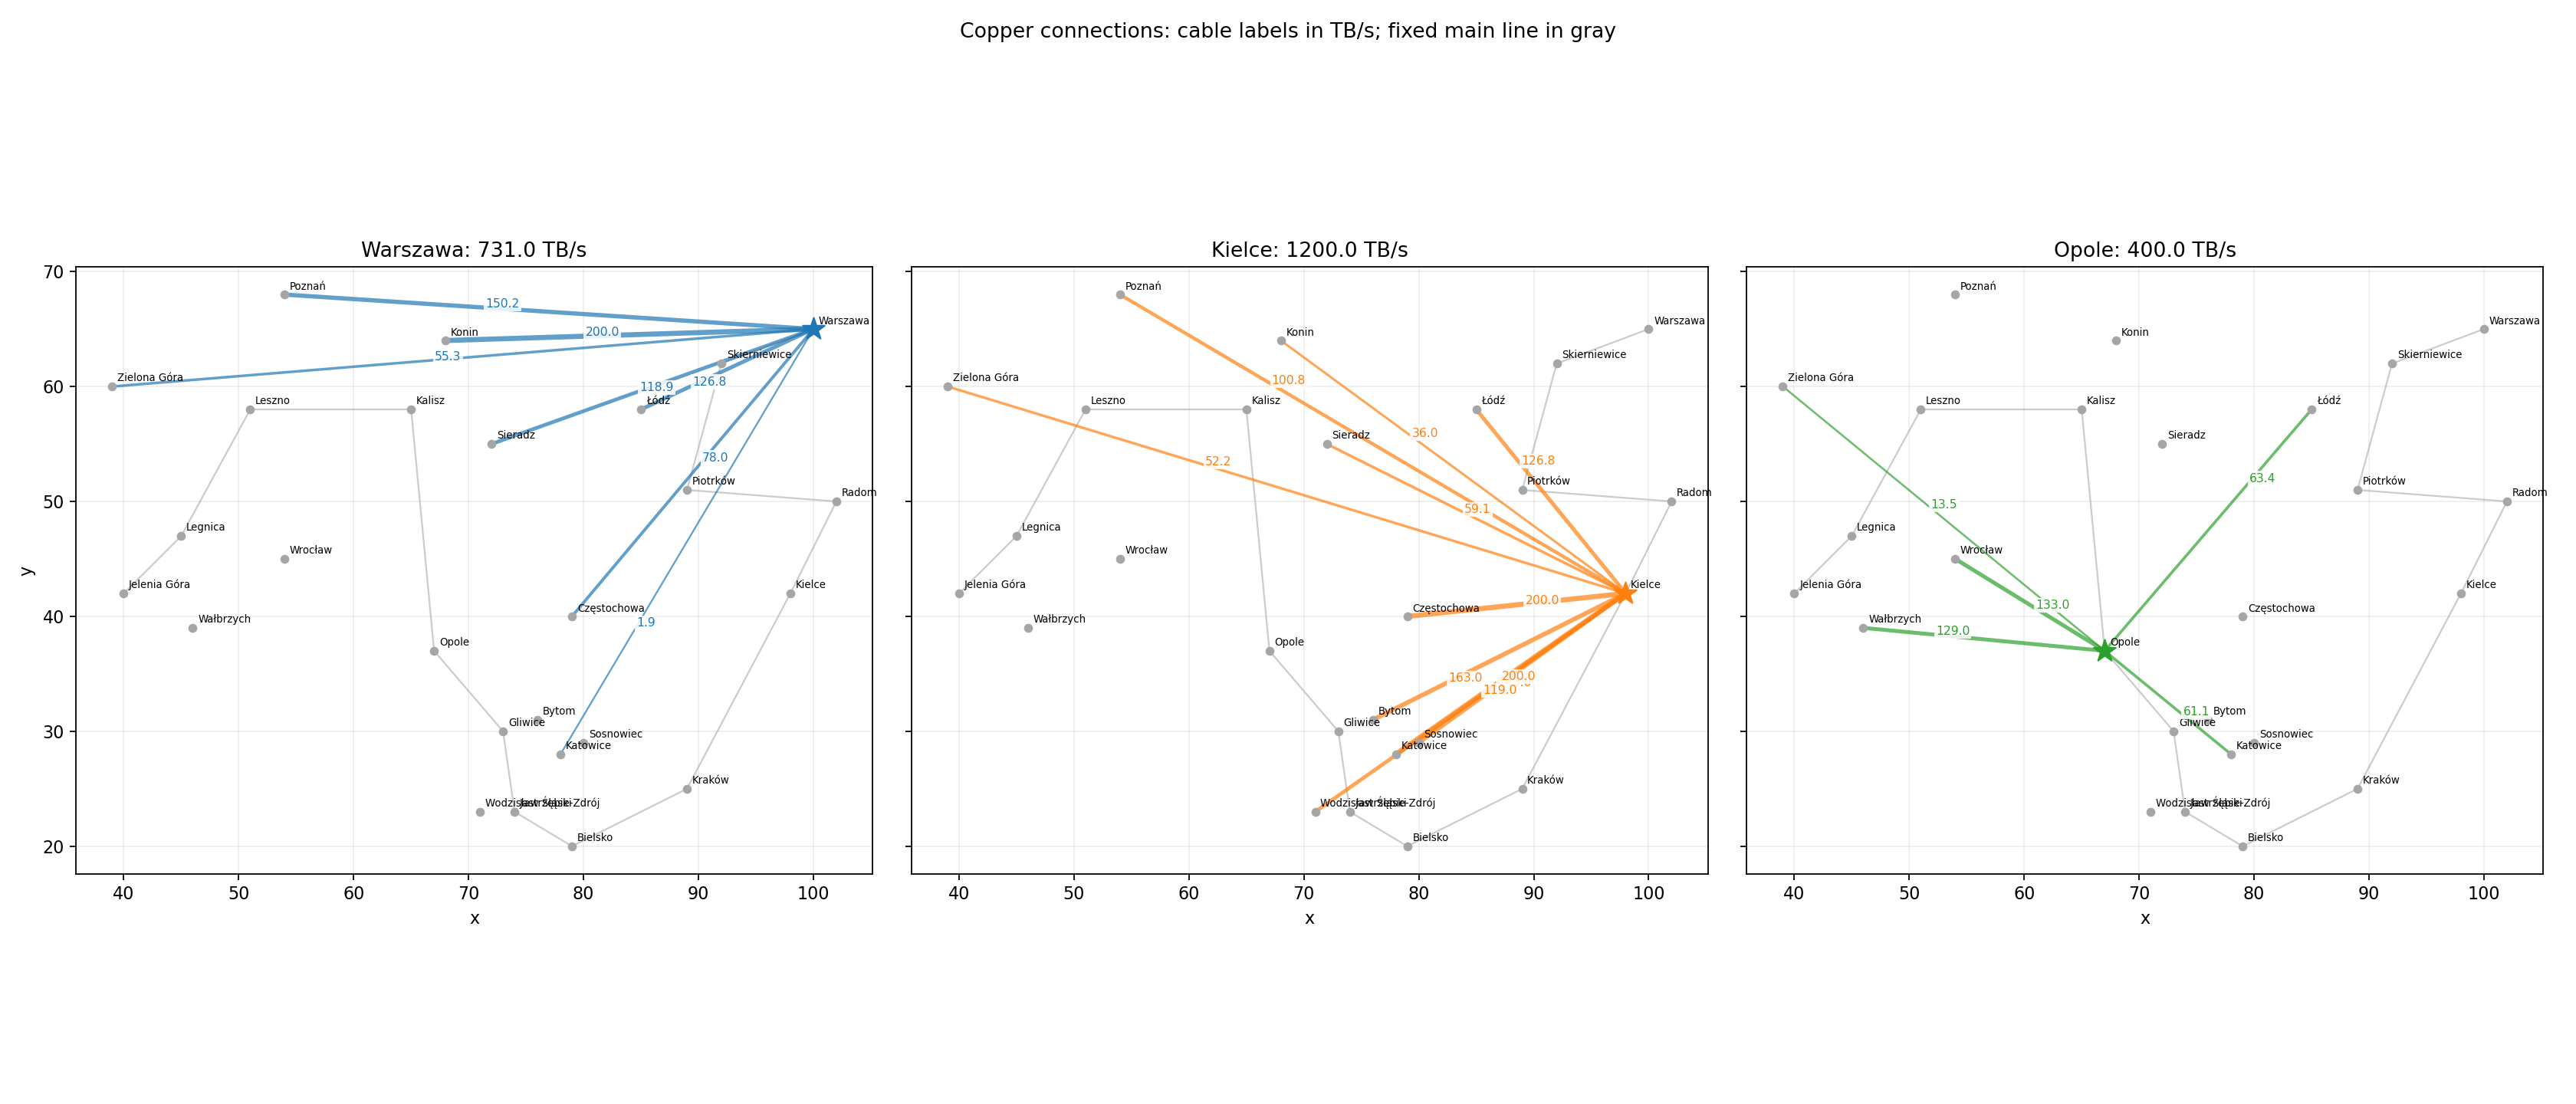
\includegraphics[width=\textwidth]{src/results/e_map.png}
\caption{Copper connections to Warszawa, Kielce, and Opole. Cable labels give capacity in TB/s, rounded to one decimal place. The main line is shown in gray.}
\label{fig:copper-map}
\end{figure}

The checker \texttt{e\_check.py} reads the saved allocations and input files without importing the optimization model. It recalculates distances, cable bounds, and costs, and verifies demand satisfaction for all 12 cities, all 36 cable bounds, station capacities, and the Łódź 40\% rule. It also checks that city--station pairs are complete and unique and that the total cost agrees with the exported summary. All these checks passed using the unrounded results.

This checker provides a separate implementation of the verification calculations, but it was generated with knowledge of the formulation. It therefore does not establish the blind AI checker generation requested by the assignment.
\textit{To be completed by the authors: obtain a checker using only the case text and solution-file format, without showing the model, and record its prompt, results, and any disagreements in the AI log.}

\subsection{Explanation using dual values}
One feature to investigate is that Poznań receives no capacity from Opole even though Opole is its nearest switching station. Station capacity constraints couple decisions across cities, so distance alone does not determine an allocation. A full explanation should use the exported dual values and cable bounds to establish why the chosen allocation minimizes total cost.

\textit{To be completed by the authors: first write your own explanation of a surprising feature using the dual values in \texttt{e\_duals.csv}. Then ask AI to assess that explanation and report whether it agreed, including any corrections and their reasons.}

\section{Sensitivity analysis}
\label{sec:sensitivity}
The main line is held fixed throughout the sensitivity analysis. Only the copper connection model is reoptimized. Calculations are implemented in \texttt{f\_sensitivity.py}; demand scenarios are saved in \texttt{f\_konin.csv} and the basis analysis in \texttt{f\_summary.json}.

\subsection{Uncertainty in Konin's demand}
The baseline demand for Konin is 236 TB/s, and the baseline copper connection cost is 66,696,434.43 EUR. To examine possible forecasting errors in either direction, the demand was decreased and increased by 10\% and 20\%, with all other input parameters fixed. Each scenario was solved to optimality rather than relying only on an extrapolated shadow price.

\begin{table}[htbp]
\centering
\small
\begin{tabular}{rrrr}
\toprule
Demand change & Demand (TB/s) & Total cost (EUR) & Cost change (EUR)\\
\midrule
$-20\%$ & 188.8 & 64,974,704.92 & $-1,721,729.51$\\
$-10\%$ & 212.4 & 65,802,810.89 & $-893,623.54$\\
$0\%$ & 236.0 & 66,696,434.43 & 0.00\\
$+10\%$ & 259.6 & 67,590,057.97 & $+893,623.54$\\
$+20\%$ & 283.2 & 68,483,681.51 & $+1,787,247.08$\\
\bottomrule
\end{tabular}
\caption{Reoptimized connection costs for changes in Konin's demand. Cost changes are relative to the baseline.}
\label{tab:konin-sensitivity}
\end{table}

A 10\% demand error changes total cost by approximately 1.340\% in either direction. A 20\% increase raises cost by 2.680\%, while a 20\% decrease reduces cost by 2.581\%. Thus, the effect of the larger forecasting error is asymmetric.

The baseline shadow price of Konin's demand constraint is approximately 37,865.404 EUR per additional TB/s. The allowable RHS interval for the analyzed basis is
\[
200\le q_{\text{Konin}}\le295.135757.
\]
Within this interval, the optimal cost is predicted by
\[
Z(q)=Z_0+37{,}865.404\,(q-236),
\]
where $Z_0$ is the baseline cost. The $-10\%$, $+10\%$, and $+20\%$ scenarios lie inside the interval, and their reoptimized costs agree with the shadow-price predictions using unrounded values. The $-20\%$ scenario lies below the interval, so the baseline shadow price cannot be extrapolated to it. Reoptimization gives the cost in Table~\ref{tab:konin-sensitivity}; the decrease is not symmetric with the $+20\%$ increase because the basis changes.

\subsection{Sensitivity to the value of $\pi$}
Changing $\pi$ alters several distance-dependent cable limits simultaneously. Individual RHS sensitivity ranges assume that only one RHS changes and therefore do not directly provide the required simultaneous interval.

For this analysis, the combined cable bound is expressed as two separate inequalities,
\[
f_{is}\le200,\qquad f_{is}\le2\pi a_{is},
\qquad a_{is}=\min(35,70-d_{is}).
\]
This is equivalent to the original capacity restriction, but makes the changing RHS values linear in $\pi$. A baseline primal simplex basis is obtained at $\pi_0=3.141592654$ and saved in \texttt{f\_baseline.bas}.

Let $B$ be the baseline basis matrix, including basic slack-variable columns, and let $h$ be the vector of RHS derivatives with respect to $\pi$. The basic variables satisfy
\[
x_B(\pi)=x_B(\pi_0)+(\pi-\pi_0)B^{-1}h.
\]
All variables in this representation are nonnegative and have no finite upper bounds; cable upper limits are represented by constraint rows. The interval is determined by requiring every basic variable to remain nonnegative. The objective coefficients and constraint matrix remain fixed, so reduced costs are unchanged and the baseline basis remains optimal while it remains feasible.

For the analyzed basis, the resulting interval is
\[
\boxed{2.932616532\le\pi\le3.196822028.}
\]
At the lower endpoint, the slack in the Poznań--Kielce distance-dependent capacity constraint reaches zero. At the upper endpoint, the capacity on the Katowice--Warszawa cable reaches zero. The endpoints are included: the basis remains feasible and optimal there, although it becomes degenerate.

During development, the calculation was validated by reoptimizing at the baseline, an interior point, both endpoints, and points $10^{-4}$ outside each endpoint. Within the interval, the feasible baseline-basis solution has the same objective as the reoptimized LP. Outside the interval, at least one baseline basic variable becomes negative, so that basis is no longer feasible. The interval refers specifically to the saved basis of the formulation with separate cable limits; equivalent formulations or alternative optimal bases may have different basis sensitivity intervals. The simplified script retains the exact basis calculation and omits these repeated validation solves. Cable allocations and the objective value can change inside the interval even though the basis remains optimal. Common approximations such as $\pi=3.14$ and $\pi=3.1416$ lie within the interval and therefore preserve the analyzed basis.

\end{document}
